\documentclass[10pt]{article}
\usepackage{graphicx,tabularx,array,geometry,tikz,pgfplots,amsmath,bbding,framed,enumitem,graphicx,wrapfig,multicol,listings,empheq,caption,float}
\usepackage{color} %red, green, blue, yellow, cyan, magenta, black, white
\definecolor{mygreen}{RGB}{28,172,0} % color values Red, Green, Blue
\definecolor{mylilas}{RGB}{170,55,241}
\usepackage[makeroom]{cancel}
\usepackage[utf8]{inputenc}
\usepackage[english]{babel}
\usepackage[nottoc]{tocbibind}

\setlength{\parskip}{2ex} %--skip lines between paragraphs
\setlength{\parindent}{0pt} %--don't indent paragraphs
\lstset{language=Matlab,%
  %basicstyle=\color{red},
  breaklines=true,%
  morekeywords={matlab2tikz},
  keywordstyle=\color{blue},%
  morekeywords=[2]{1}, keywordstyle=[2]{\color{black}},
  identifierstyle=\color{black},%
  stringstyle=\color{mylilas},
  commentstyle=\color{mygreen},%
  showstringspaces=false,%without this there will be a symbol in the places where there is a space
  numbers=left,%
  numberstyle={\tiny \color{black}},% size of the numbers
  numbersep=9pt, % this defines how far the numbers are from the text
  emph=[1]{for,end,break},emphstyle=[1]\color{red}, %some words to emphasise
  %emph=[2]{word1,word2}, emphstyle=[2]{style},    
}
\geometry{
 total={210mm,297mm},
 left=20mm,
 right=20mm,
 top=20mm,
 bottom=20mm,
 }
 \pgfplotsset{compat=1.12}
%-- Commands for header
\newcommand*\widefbox[1]{\fbox{\hspace{2em}#1\hspace{2em}}}
\renewcommand{\title}[1]{\textbf{#1}\\}
\renewcommand{\line}{\begin{tabularx}{\textwidth}{X>{\raggedleft}X}\hline\\\end{tabularx}\\[-0.5cm]}
\newcommand{\leftright}[2]{\begin{tabularx}{\textwidth}{X>{\raggedleft}X}#1%
\end{tabularx}\\[-0.5cm]}

%\linespread{2} %-- Uncomment for Double Space
\begin{document}

\title{Final 22.212 Report\qquad Amelia Trainer }
\line\\
\leftright{\today}{ }%-- left and right positions in the header
~\par

%%%%%%%%%%%%%%%%%%%%%%%%%%%%%%%%%%%%%%%%%%%%%%%%%%%%%%%%%%%%%%%%%%%%%%%%%%%%%%%
%%%%%%%%%%%%%%%%%%%%%%%%%%%%%%%%%%%%%%%%%%%%%%%%%%%%%%%%%%%%%%%%%%%%%%%%%%%%%%%
\section{Introduction}
%%%%%%%%%%%%%%%%%%%%%%%%%%%%%%%%%%%%%%%%%%%%%%%%%%%%%%%%%%%%%%%%%%%%%%%%%%%%%%%
%%%%%%%%%%%%%%%%%%%%%%%%%%%%%%%%%%%%%%%%%%%%%%%%%%%%%%%%%%%%%%%%%%%%%%%%%%%%%%%
Due to the overwhelming size and number of necessary nuclear cross section data files needed for a reactor calculation, adopting a multigroup cross section approach is extremely popular for determinisitc neutronics calculations. Cross section resonances greatly impact the flux by creating depressions, since neutrons with energy equal to that of the resonance are highly likely to experience the resonance's corresponding reaction. In most reactors where neutrons are born fast and are slowed down through the resonance range, this effect relating to neutron flux depressions near resonances (i.e. self-shielding) is extremely important to characterize.\par
One approach to modeling the problem of resonance self-shielding is called equivalence in dilution, which requires the construction of a dilution table. Important parameters (e.g. cross sections, resonance integrals) are tabulated against dilution or background cross sections. In doing so, a homogeneous geometry can be treated identically to a heterogeneous problem if they both have the same background cross section $\sigma_0$ used to look up the tabulated values. Wigner, Bell-Wigner, Carlvik and Roman are a few well-known types of approximations that can be used to achieve an equivalence in dilution relationship. When considering a lattice system, where pins ``shadow'' each other and complicate the pin-to-pin collision probabilities, a Dancoff factor can be used. The goal of this paper is to discuss an alternative to the aforementioned equivalence methods, called Tone's method. Tone's method is an alternate way of calculating a heterogeneous system's background cross section, but does so in a way that iteratively calculates the pin-to-pin collision probabilities, thus eliminating the need for a separately defined Dancoff factor. 


%%%%%%%%%%%%%%%%%%%%%%%%%%%%%%%%%%%%%%%%%%%%%%%%%%%%%%%%%%%%%%%%%%%%%%%%%%%%%%%
%%%%%%%%%%%%%%%%%%%%%%%%%%%%%%%%%%%%%%%%%%%%%%%%%%%%%%%%%%%%%%%%%%%%%%%%%%%%%%%
\section{Background}
%%%%%%%%%%%%%%%%%%%%%%%%%%%%%%%%%%%%%%%%%%%%%%%%%%%%%%%%%%%%%%%%%%%%%%%%%%%%%%%
%%%%%%%%%%%%%%%%%%%%%%%%%%%%%%%%%%%%%%%%%%%%%%%%%%%%%%%%%%%%%%%%%%%%%%%%%%%%%%%



%%%%%%%%%%%%%%%%%%%%%%%%%%%%%%%%%%%%%%%%%%%%%%%%%%%%%%%%%%%%%%%%%%%%%%%%%%%%%%%
\subsection{Narrow Resonance Approximation}
%%%%%%%%%%%%%%%%%%%%%%%%%%%%%%%%%%%%%%%%%%%%%%%%%%%%%%%%%%%%%%%%%%%%%%%%%%%%%%%

\subsubsection{Neutron Slowing Down in Homogeneous System}
We start with the Boltzmann Equation.
\begin{equation}\Sigma_{t}(E)\phi(E)=\int_{0}^{\infty}\Sigma_{s}\left(E^{\prime}\rightarrow E\right)\phi\left(E^{\prime}\right)\mathrm{d}E^{\prime}+\frac{\chi(E)}{k_{eff}}\int_{0}^{\infty}v\Sigma_{f}\left(E^{\prime}\right)\phi\left(E^{\prime}\right)\mathrm{d}E^{\prime}\end{equation}

We're working in the resonance region, where scattering is the main form of neutrons slowing down, which allows us to get rid of our fission term, simplifying the Boltzmann Equation to
\begin{equation}\Sigma_{t}(E)\phi(E)=\int_{0}^{\infty}\Sigma_{s}\left(E^{\prime}\rightarrow E\right)\phi\left(E^{\prime}\right)\mathrm{d}E^{\prime}.\end{equation}

We represent the macroscopic cross sections as their constituents: number density $N$, microscopic cross section $\sigma$, and probability $P(E'\rightarrow E)$ of a scattering event resulting in energy transition to $E$ from $E'$.
\begin{equation}\left(\sum\limits_{k}N_{k}\sigma_{t,k}(E)\right)\phi(E)=\sum\limits_{k}\int_{E}^{E/\alpha_{k}}N_{k}\sigma_{s,k}\left(E^{\prime}\right)\phi\left(E^{\prime}\right)P(E'\rightarrow E)\mathrm{d}E^{\prime}\end{equation}
Recalling that 
\begin{equation}P(E'\rightarrow E)dE'=\frac{1}{(1-\alpha_k)E'}dE',\end{equation}
we can further simplify the scattering kernel, bringing the equation to
\begin{equation}\left(\sum\limits_{k}N_{k}\sigma_{t,k}(E)\right)\phi(E)=\sum\limits_{k}\frac{1}{1-\alpha_{k}}\int_{E}^{E/\alpha_{k}}\frac{1}{E'}N_{k}\sigma_{s,k}\left(E^{\prime}\right)\phi\left(E^{\prime}\right)\mathrm{d}E^{\prime}\end{equation}


Note that we are currently prevented from further simplifying the above integral, due to the energy dependence of $\sigma_{s,k}(E')$ and $\phi(E')$. This prompts us to make two additional approximations: the Narrow Resonance (NR) approximation, and the $1/E$ flux approximation.\par

Assuming a sufficiently thin resonance allows us to approximate that every scattering event will miss the resonance. We thus assume that the scattering kernel is simply equal to the potential scattering cross section $\sigma_{pot}$, which is constant in energy. Doing so eliminates the energy dependence of the cross section, leaving us with
\begin{equation}\sum\limits_{k}\frac{1}{1-\alpha_{k}}\int_{E}^{E/\alpha_{k}}\frac{1}{E'}N_{k}\sigma_{s,k}\left(E^{\prime}\right)\phi\left(E^{\prime}\right)\mathrm{d}E^{\prime}=\sum\limits_{k}\frac{N_k\sigma_{pot,k}}{1-\alpha_{k}}\int_{E}^{E/\alpha_{k}}\frac{1}{E'}\phi\left(E^{\prime}\right)\mathrm{d}E^{\prime}.\end{equation}
  Now an approximation of the flux is all that is needed to simplify the integral to a solvable form. We assume $\phi(E)\approx1/E$ for the scalar flux, which allows 
\begin{align}\sum\limits_{k}\frac{1}{1-\alpha_{k}}\int_{E}^{E/\alpha_{k}}\frac{1}{E'}N_{k}\sigma_{s,k}\left(E^{\prime}\right)\phi\left(E^{\prime}\right)\mathrm{d}E^{\prime} 
  =&\sum\limits_{k}\frac{N_k\sigma_{pot,k}}{1-\alpha_{k}}\int_{E}^{E/\alpha_{k}}\frac{1}{(E')^2}\mathrm{d}E^{\prime}\\
  = &\sum\limits_{k}\frac{N_{k}\sigma_{pot,k}}{1-\alpha_{k}}\left(\frac{1}{E}-\frac{\alpha_k}{E}\right)\\
    =&\sum\limits_k\frac{N_{k}\sigma_{pot,k}}{E}
\end{align}


\begin{equation}\sum\limits_{k}\frac{1}{1-\alpha_{k}}\int_{E}^{E/\alpha_{k}}\frac{1}{E'}N_{k}\sigma_{s,k}\left(E^{\prime}\right)\phi\left(E^{\prime}\right)\mathrm{d}E^{\prime} =\sum\limits_k\frac{N_{k}\sigma_{pot,k}}{E}\label{eq:NRConclusion}\end{equation}











\subsubsection{Neutron Slowing Down in Isolated, Heterogeneous System}
Consider a neutron slowing down in a two-region heterogeneous problem, where $f,m$ represent fuel and moderator, respectively. Note that while the following discussion is based on a two region problem, it can be extended to accommodate more complicated geometries.
\begin{align}\Sigma_{t,f}(E)\phi_{f}(E)V_{f}=P_{f\rightarrow f}(E)V_{f}&\int_{0}^{\infty}\Sigma_{s,f}\left(E^{\prime}\rightarrow E\right)\phi_{f}\left(E^{\prime}\right)dE^{\prime}\\ + P_{m\rightarrow f}(E)V_{m}&\int_{0}^{\infty}\Sigma_{s,m}\left(E^{\prime}\rightarrow E\right)\phi_{m}\left(E^{\prime}\right)dE^{\prime}\end{align}

We separate the macroscopic cross section for scattering to energy $E$ into its number density $N$, microscopic cross section $\sigma_s$, and probability of energy change $P(E'\rightarrow E)$, to rewrite the balance equation as 
\begin{align}\Sigma_{t,f}(E)\phi_{f}(E)V_{f}=P_{f\rightarrow f}(E)V_{f}&\int_{0}^{\infty}\sum\limits_{k\in f}N_k\sigma_{s,k}P(E'\rightarrow E)\phi_{f}\left(E^{\prime}\right)dE^{\prime}\\ + P_{m\rightarrow f}(E)V_{m}&\int_{0}^{\infty}\sum\limits_{k\in m}N_k\sigma_{s,k}P\left(E^{\prime}\rightarrow E\right)\phi_{m}\left(E^{\prime}\right)dE^{\prime}\end{align}

Recalling the energy distribution of a single neutron scattering collision is 
\begin{equation}P(E'\rightarrow E)=\frac{1}{(1-\alpha)E}~\mbox{for }\alpha E\leq E'\leq E,\end{equation}
we can further simplify the balance equation to be

\begin{align}\Sigma_{t,f}(E)\phi_{f}(E)V_{f} = P_{f\rightarrow f}(E)V_{f}\sum\limits_{k\in f}&\int_{E}^{E/\alpha_{k}}\frac{N_{k}\sigma_{s,k}\left(E^{\prime}\right)\phi_{f}\left(E^{\prime}\right)}{\left(1-\alpha_{k}\right)E^{\prime}}dE^{\prime}  \\
+ P_{m\rightarrow f}(E)V_{m}\sum\limits_{k\in m}&\int_{E}^{E/\alpha_{k}}\frac{N_{k}\sigma_{s,k}\left(E^{\prime}\right)\phi_{m}\left(E^{\prime}\right)}{\left(1-\alpha_{k}\right)E^{\prime}}dE^{\prime}.\label{eq:hetero-balance}\end{align}


Eq.~\ref{eq:NRConclusion} can be used to simplify Eq.~\ref{eq:hetero-balance}, yielding


\begin{equation}\Sigma_{t,f}(E)\phi_{f}(E)V_{f}=\frac{1}{E}\Big(P_{f\rightarrow f}(E)V_{f}\Sigma_{pot,f}+P_{m\rightarrow f}(E)V_{m}\Sigma_{pot,m}\Big)\end{equation}
\begin{equation}\phi_{f}(E)=\frac{P_{f\rightarrow f}(E)V_f\Sigma_{pot,f}+P_{m\rightarrow f}(E)V_m\Sigma_{pot,m}}{E\Sigma_{t,f}(E)V_f}\end{equation}

Note that while this result is derived using a two-region problem, it can be extended to solve for a flux in region $i\in N$, which is dependent on all $j\in N$ regions:

\begin{equation}\phi_{i}(E)=\frac{1}{E}\sum\limits_j\frac{P_{j\rightarrow i}(E)V_{j}\Sigma_{pot,j}}{\Sigma_{t,i}(E)V_{i}}\label{eq:resultFromHetero}\end{equation}




%%%%%%%%%%%%%%%%%%%%%%%%%%%%%%%%%%%%%%%%%%%%%%%%%%%%%%%%%%%%%%%%%%%%%%%%%%%%%%%
  \subsection{Tone's Method}\label{sec:tone}
%%%%%%%%%%%%%%%%%%%%%%%%%%%%%%%%%%%%%%%%%%%%%%%%%%%%%%%%%%%%%%%%%%%%%%%%%%%%%%%
We start with the result from Eq.~\ref{eq:resultFromHetero}, which defines the energy dependent neutron flux in region $i$ on the collision probabilities of going from all regions $j$ to region $i$. Tone's method approximates the energy dependence of $P_{j\rightarrow i}(E)$ and $\Sigma_{t,i}(E)$ to be group constant, such that 
\begin{equation}\frac{P_{j\rightarrow i}(E)}{\Sigma_{t,i}(E)}=\alpha_{i}(E)\frac{P_{j\rightarrow i,g}}{\Sigma_{t,i,g}}.\label{eq:tonesApprox}\end{equation}
  Note that while the collision probabilities and total cross sections are approximated to be group constants, there is included a fine energy factor $\alpha_i(E)$. However, note that this fine energy term is \textbf{only dependent on the region the neutrons are going into}. This is a major assumption, since in reality the actual collision probability is dependent on other regions (including the source region). Approximating $\alpha(E)\approx\alpha_i(E)$ is, however, a likely better approximation than $\alpha(E)\approx\alpha_j(E)$, since region $i$ is where the incoming neutrons induce reactions (e.g. fission, absorption).

Using Eq.~\ref{eq:tonesApprox} in Eq.~\ref{eq:resultFromHetero} elimintes the fine energy dependence of the collision probabilities and cross sections,

\begin{equation}\phi_{i}(E)=\frac{\alpha_i(E)}{E\Sigma_{t,i,g}V_i}\sum\limits_j\Big(P_{j\rightarrow i,g}V_{j}\Sigma_{pot,j}\Big)\label{eq:phiWithAlpha}\end{equation}
Attaining a cleaner representation of $\phi_i(E)$ requires getting a better description of $\alpha_i(E)$. Doing so requires use of two tools:
% We'll use two tools to aid us in the derivation
  \begin{enumerate}
    \item Reciprocity relation
      \begin{equation*}P_{j\rightarrow i}(E)V_{j}\Sigma_{t,j}(E)=P_{i\rightarrow j}(E)V_{i}\Sigma_{t,i}(E)\end{equation*}
        \begin{equation}P_{i\rightarrow j}(E)=\frac{P_{j\rightarrow i}(E)V_{j}\Sigma_{t,j}(E)}{V_{i}\Sigma_{t,i}(E)}\label{eq:reciprocity}\end{equation}
    \item Probabilities normalize to 1
      \begin{equation}\sum\limits_{j}P_{i\rightarrow j}(E)=1\label{eq:probSum}\end{equation}
  \end{enumerate}


The reciprocity relation (Eq.~\ref{eq:reciprocity}) can be combined with the normalization statement (Eq.~\ref{eq:probSum}) to get
\begin{equation}\sum\limits_{j}\left(\frac{P_{j\rightarrow i}(E)V_{j}\Sigma_{t,j}(E)}{V_{i}\Sigma_{t,i}(E)}\right)=1.\label{eq:endOfReciprocity}\end{equation}
The fine energy dependence of the collision probabilities and the total cross sections can be approximated using Eq.~\ref{eq:tonesApprox}, which can be used to isolate $\alpha_i(E)$,
\begin{equation}\frac{\alpha_i(E)}{V_i\Sigma_{t,i,g}}\sum\limits_{j}\Big(P_{j\rightarrow i,g}V_{j}\Sigma_{t,j}(E)\Big)=1\end{equation}
\begin{equation}\alpha_i(E)=\frac{V_i\Sigma_{t,i,g}}{\sum\limits_{j}\Big(P_{j\rightarrow i,g}V_{j}\Sigma_{t,j}(E)\Big)}.\end{equation}



Now having a formulation for $\alpha_i(E)$, we can rewrite Eq.~\ref{eq:phiWithAlpha} as


\begin{equation}\phi_{i}(E)=\frac{1}{E\Sigma_{t,i,g}V_i}\frac{V_i\Sigma_{t,i,g}}{\sum\limits_{j}\left(P_{j\rightarrow i,g}V_{j}\Sigma_{t,j}(E)\right)}\sum\limits_j\Big(P_{j\rightarrow i,g}V_{j}\Sigma_{pot,j}\Big)\end{equation}
\begin{equation}\phi_{i}(E)=\frac{1}{E}\frac{\sum\limits_j\Big(P_{j\rightarrow i,g}V_{j}\Sigma_{pot,j}\Big)}{\sum\limits_{j}\left(P_{j\rightarrow i,g}V_{j}\Sigma_{t,j}(E)\right)}\end{equation}
  The two macroscopic cross sections, $\Sigma_{t,j}$ and $\Sigma_{pot,k}$, are broken into their number density $N$ and microscopic cross section $\sigma$ constituents. They are also separated into resonant and non-resonant nuclides\footnote{Tone's method, like other equivalence methods, consider one nuclide at a time to be resonant, and assumes all other are non-resonant (constant). If there is more than one resonant nuclide in the material, they take turns beign considered resonant.}. 
\begin{equation}\phi_{i}(E)=\frac{1}{E}\frac{\sum\limits_j\left(P_{j\rightarrow i,g}V_{j}\left(N_{r,j}\sigma_{pot,r}+\sum\limits_{k\neq r}N_{k,j}\sigma_{pot,k}\right)\right)}{\sum\limits_{j}\left(P_{j\rightarrow i,g}V_{j}\left(N_{r,j}\sigma_{r,t}(E)+\sum\limits_{k\neq r}N_{k,j}\sigma_{t,k}(E)\right)\right)}\end{equation}
  The total cross section for all non-resonant nuclides $\sigma_{t,k\neq r}$ is approximated to be constant in energy, and equal to the potential scattering cross section $\sigma_{pot,k\neq r}$, as is typical treatment for non-resonant nuclides in equivalence theory. Doing so is valid, since this energy-independent potential scattering is dominant for nonresonant nuclides in the resonance energy range~\cite{ch9}.
\begin{equation}\phi_{i}(E)\approx\frac{1}{E}\frac{\sum\limits_j\left(P_{j\rightarrow i,g}V_{j}\left(N_{r,j}\sigma_{pot,r}+\sum\limits_{k\neq r}N_{k,j}\sigma_{pot,k}\right)\right)}{\sum\limits_{j}\left(P_{j\rightarrow i,g}V_{j}\left(N_{r,j}\sigma_{r,t}(E)+\sum\limits_{k\neq r}N_{k,j}\sigma_{pot,k}\right)\right)}\label{eq:almost}\end{equation}


Mild rearrangement of terms in Eq.~\ref{eq:almost} yields
\begin{equation}\phi_{i}(E)=\frac{1}{E}\frac{\sigma_{pot,r}+\left(\sum\limits_jP_{j\rightarrow i,g}V_{j}\sum\limits_{k\neq r}N_{k,j}\sigma_{pot,k}\Big/\sum\limits_jP_{j\rightarrow i,g}V_{j}N_{r,j}\right)}{\sigma_{r,t}(E)+\Big(\sum\limits_{j}P_{j\rightarrow i,g}V_{j}\sum\limits_{k\neq r}N_{k,j}\sigma_{pot,k}\Big/\sum\limits_{j}P_{j\rightarrow i,g}V_{j}N_{r,j}\Big)}\end{equation}
which can is the same in form as the NR approximation for a homogeneous system, only with a different defintion of background cross section. The final form of the flux equations from Tone's method are
\begin{equation}\boxed{\phi_i(E)=\frac{1}{E}\frac{\sigma_{pot,r}+\sigma_{0}}{\sigma_{t,r}(E)+\sigma_{0}}~\mbox{where }\sigma_{0}=\frac{\sum\limits_j\sum\limits_{k\neq r}P_{j\rightarrow i,g}V_{j}N_{k,j}\sigma_{pot,k}}{\sum\limits_jP_{j\rightarrow i,g}V_{j}N_{r,j}}.}\label{eq:Tones}\end{equation}





%%%%%%%%%%%%%%%%%%%%%%%%%%%%%%%%%%%%%%%%%%%%%%%%%%%%%%%%%%%%%%%%%%%%%%%%%%%%%%%
%%%%%%%%%%%%%%%%%%%%%%%%%%%%%%%%%%%%%%%%%%%%%%%%%%%%%%%%%%%%%%%%%%%%%%%%%%%%%%%
\section{Method}
%%%%%%%%%%%%%%%%%%%%%%%%%%%%%%%%%%%%%%%%%%%%%%%%%%%%%%%%%%%%%%%%%%%%%%%%%%%%%%%
%%%%%%%%%%%%%%%%%%%%%%%%%%%%%%%%%%%%%%%%%%%%%%%%%%%%%%%%%%%%%%%%%%%%%%%%%%%%%%%



%%%%%%%%%%%%%%%%%%%%%%%%%%%%%%%%%%%%%%%%%%%%%%%%%%%%%%%%%%%%%%%%%%%%%%%%%%%%%%%
\subsection{Overview}\label{recipe}
%%%%%%%%%%%%%%%%%%%%%%%%%%%%%%%%%%%%%%%%%%%%%%%%%%%%%%%%%%%%%%%%%%%%%%%%%%%%%%%
Tone's Method can be appropriately performed using the following steps~\cite{ch9}:

      \begin{enumerate}
        \item \textbf{Assume initial $\sigma_0$ for resonance nuclides, using conventional equivalence methods}\\
  For a heterogeneous system, our background cross section is comprised of a material-component and a geometry-component.
\begin{equation}\sigma_{0,r}=\sigma_{0,f}+\frac{\Sigma_e}{N_r}=\sum_{k\neq r}\frac{N_k\sigma_{s,k}}{N_r}+\frac{\Sigma_e}{N_r}\label{eq:conventional}\end{equation}
Note that for Tone's method, the initial estimate for background cross section is not too important since it'll iterate out anyway.

        \item \textbf{Evaluate the effective cross sections of resonance nuclides using the conventional equivalence theory}
          The GROUPR module from the NJOY nuclear data processing code was uesd to create a dilution table, which allows users to obtain cross section values for a heterogeneous problem by tabulating effective cross sections $\sigma_{eff}$ for various dilution cross ections. 
           Equivalence theory involved the creation of a dilution table, where relevant parameters (e.g. cross sections, resonance integrals) are tabulated against background cross sections. The table is created asssuming a homogeneous geometry, but can be used to solve heterogeneous problems if the background cross sections used are chosen to appropriately reflect the heterogeneity of the problem. \par
           Construction of this table is performed using the GROUPR module of the NJOY nuclear data processing code. Once a background cross section $\sigma_{0,r}$ is computed using Eq.~\ref{eq:conventional} or Eq.~\ref{eq:Tones}, the corresponding cross sections can be looked up in the dilution table.
         \item \textbf{Evaluate group-wise collision probability using effective cross sections}
           The collision probability $P_{j\rightarrow i,g}$ is computed for each group using a Monte Carlo simlution, where neutrons are born in a pincell and are tracked until thei
         \item \textbf{Update the background cross section using Eq.~\ref{eq:Tones}.}

         \item \textbf{Repeat until convergence.}
      \end{enumerate}




%%%%%%%%%%%%%%%%%%%%%%%%%%%%%%%%%%%%%%%%%%%%%%%%%%%%%%%%%%%%%%%%%%%%%%%%%%%%%%%
\subsection{Problem Selection}
%%%%%%%%%%%%%%%%%%%%%%%%%%%%%%%%%%%%%%%%%%%%%%%%%%%%%%%%%%%%%%%%%%%%%%%%%%%%%%%

\subsubsection{Equivalence in Dilution Table}

Effective cross sections for U-238 capture is plotted in Fig.~\ref{fig:njoyDil} for various background cross sections, along with the corresponding pointwise data. Note that over the resonances, the effective capture cross section values can vary greatly for different background cross sections. Thus ensuring that the $\sigma_0$ grid used in the dilution table must be adequately resolved. This dependency of effective cross sections on background cross section is further explored in Fig.~\ref{fig:dependencyOnBackground}, which plots $\sigma_a$ against $\sigma_0$, for various energy groups in the resonance range. 

\begin{figure}[H]
  \begin{center}
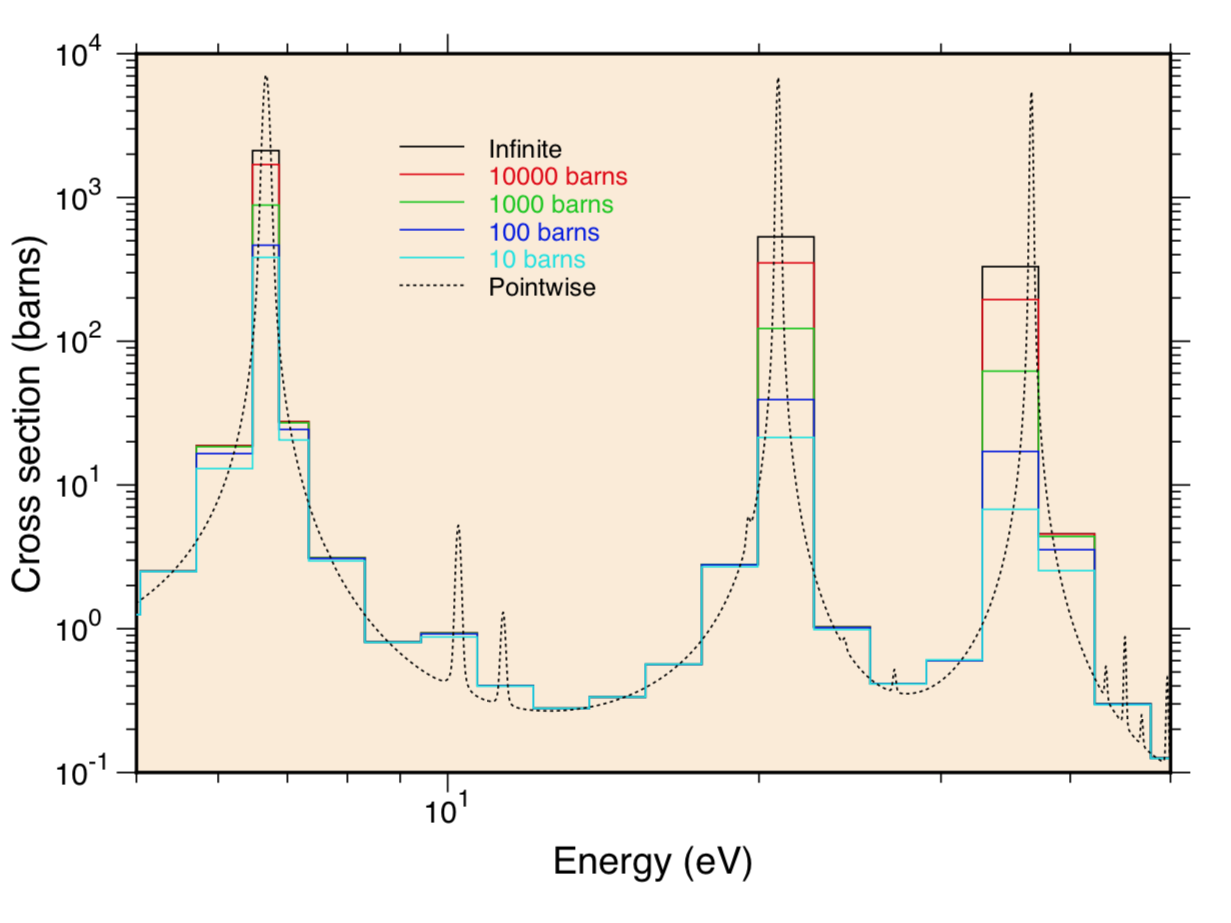
\includegraphics[width=0.6\textwidth]{njoyGroupr}
  \caption{The self-shielding effect on the first three U-238 capture resonance at room temperature in the 5-50 eV energy range. The multigroup boundaries are from the Los Alamos 187-grioup structure~\cite{njoy16}. Note that the cross sections over the resonances can change by over an order of magnitude, when calcualted using different background cross sections $\sigma_0$.}
  \label{fig:njoyDil}
  \end{center}
\end{figure}

  \begin{figure}[H]
    \begin{center}
%    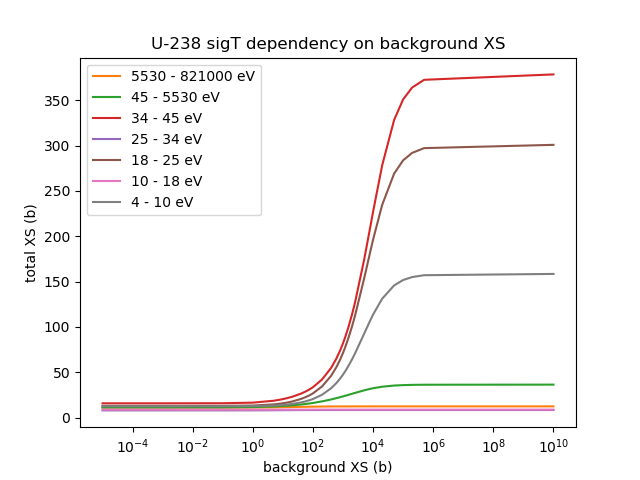
\includegraphics[width=0.55\textwidth]{U238_sigT_dependency_on_background}
    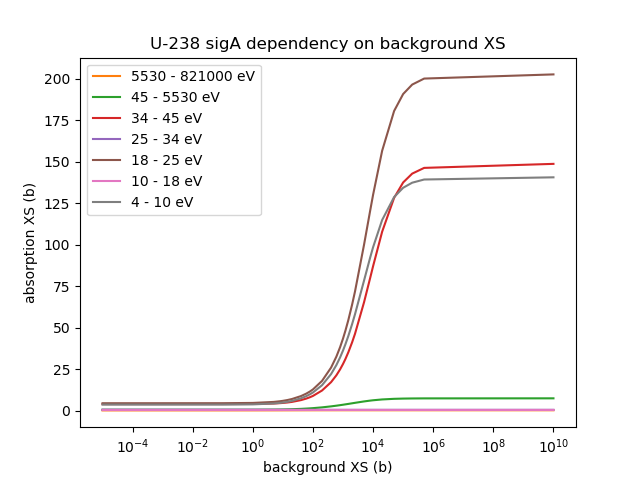
\includegraphics[width=0.7\textwidth]{U238_sigA_dependency_on_background}\\
      %\caption{Both conventional equivalence theory and Tone's method require the creation of a dilution table, so that given a background cross section $\sigma_0$, effective cross sections (e.g. $\sigma_{t,eff},\sigma_{a,eff}$) can be obtained. However, since $\sigma_0$ can span from $0\rightarrow\infty$, the dependency that the effective cross sections have on $\sigma_0$ must be analyzed, to allow for and appropriate $\sigma_0$ grid to be selected. Shown above are the $\sigma_{t,eff},\sigma_{a,eff}$ cross sections for U-238 at 300 K, plotted against $\sigma_0$. Naturally the most important effects will occur in the energy groups that contain U-238's 6.67, 20.5, and 36.6 eV resonances. Note the drastic changes to effective cross sections that occur in the $\sigma_0=10^2-10^3$ b range. The background cross section grid must thus be appropriately resolved in this range. }
      \caption{Both conventional equivalence theory and Tone's method require the creation of a dilution table, so that given a background cross section $\sigma_0$, effective cross sections (e.g. $\sigma_{a,eff}$) can be obtained. However, since $\sigma_0$ can span from $0\rightarrow\infty$, the dependency that the effective cross sections have on $\sigma_0$ must be analyzed, to allow for and appropriate $\sigma_0$ grid to be selected. Shown above are the $\sigma_{a,eff}$ cross sections for U-238 at 300 K, plotted against $\sigma_0$. Naturally the most important effects will occur in the energy groups that contain U-238's 6.67, 20.5, and 36.6 eV resonances. Note the drastic changes to effective cross sections that occur in the $\sigma_0=10^2-10^3$ b range. The background cross section grid must thus be appropriately resolved in this range. }
      \label{fig:dependencyOnBackground}
      %In order to evaluate the effective cross sections of U-238 using convenctional equivalence theory, a dilution table was created so that, given a background cross section value $\sigma_0$, microscopic cross sections (e.g. $\sigma_t,\sigma_a$) could be obtained. }
    \end{center}
  \end{figure}

Due to the observations made in Fig.~\ref{fig:dependencyOnBackground}, the following dilution cross section grid was selected:\par
$\sigma_0 =$ 1E-5 1E-3 0.1 1 5 8 10 14 20 40 60 80 100 200 400 600 800 \\
\null\qquad~\quad1000 1200 1500 2000 8000 1E4 2E4 5E4 1E5 2E5 5E5 1E10

%\begin{table}[H]
%  \begin{center}
%\begin{tabular}{|l|l|l|l|l|l|l|}\hline
%   &  &  &    &    &  &  \\\hline
%  1E-5 & 1E-3 & 0.1 & 1   & 5   & 8 &  \\\hline
%  10 & 14 & 20 & 40 & 60 & 80& \\\hline
%  100  & 200  & 400 & 600 & 800&& \\\hline
%  1000 & 1200 & 1500 & 2000 & 2500 & 5000 & 8000 \\\hline
%  1E4  & 2E4  & 5E4  & 1E5 & 2E5  & 5E5 & 10E10 \\\hline
%\end{tabular}
%    \caption{$\sigma_0$ values (in barns)  uesd for generating dilution table. Note that increased fineness in grid for values in the 10's to 1000's region. The choice to do so was due to the behavior observed in Fig.~\ref{fig:dependencyOnBackground}.}
%  \end{center}
%\end{table}






\subsubsection{Enrichment and Heterogeneity}\label{enrichment}

Recall Eq.~\ref{eq:Tones}, which defines the flux and background cross section $\sigma_0$ for Tone's method.
\begin{equation*}\phi_i(E)=\frac{1}{E}\frac{\sigma_{pot,r}+\sigma_{0}}{\sigma_{t,r}(E)+\sigma_{0}}~\mbox{where }\sigma_{0}=\frac{\sum\limits_j\sum\limits_{k\neq r}P_{j\rightarrow i,g}V_{j}N_{k,j}\sigma_{pot,k}}{\sum\limits_jP_{j\rightarrow i,g}V_{j}N_{r,j}}\tag{\ref{eq:Tones}}\end{equation*}
  Note that if all pins are identical ($N_{k,j}=N_k$, $N_{r,j}=N_r$, and $V_j=V$ for all $j$), then the background cross section reduces to 
  \begin{equation}\sigma_0=\sum\limits_{k\neq r}\frac{N_k\sigma_{pot,k}}{N_r}\end{equation}
    which is identical to the background cross section used for a homogenous, narrow resonance approximated system. Thus, in order for Tone's method to noticeably change $\sigma_0$, the pins must be sufficiently different in number density $N$ and/or volume. \par
    Once $\sigma_0$ is calculated, it will be used to look up effective cross section values $\sigma_{eff}$ in the dilution table. Because of this, the changes that Tone's method imposes will be most noticeable when $\sigma_{eff}$ values are strongly dependent on $\sigma_0$. Fig.~\ref{fig:dependencyOnBackground} suggests that a if $\sigma_0$ values were to be within the range 100-1000 b, then the changes reflected in $\sigma_{eff}$ values would be quite noticeable.\par
    Therefore, the geometry used for this project is chosen to have pins of significantly different enrichments, so that Eq.~\ref{eq:Tones} is prevented from reducing to the homogeneous representation. While considering U-238 to be the resonant nuclide, the enrichment should be adequately high so as to drive the background cross section up, making the system more dilute. The geometry used for this project is presented in Fig.~\ref{fig:geometry}. The geometry consists of a checkerboard distribution of enrichments, alternating between 90\% (red) and 4\% (yellow). The radii of all pins is 0.3918 cm, the pitches are 1.26 cm, and the outer boundary conditions are all reflective.
    
    
 \begin{figure}
    \begin{center}
      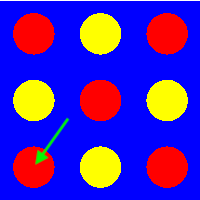
\includegraphics[width=0.3\textwidth]{full_3x3}
      \caption{Above is a schematic of the geometry used for this project. It consists of a 3x3 grid of pincells, with checkerboard enrichment. The red pins are HEU, with 90\% U-235 and 10\% U-238. The yellow pins are LEU, at 4\% U-235 and 96\% U-238. These U isotopes, along with O-16, are the only nuclides tracked in the fuel. The pin radii are identical at 0.39128 cm, and the pitch is 1.26 cm. The bottom left pin pointed to with the green arrow is the region $i$ that is singled out in Eq.~\ref{eq:Tones}. Reflective boundary conditions are used for all four sides.}
      \label{fig:geometry}
    \end{center}
\end{figure}




  \section{Results of Tone's Method}
  The procedure describing Tone's method presented in Sec.~\ref{recipe} was performed for the problem specifications described in Sec.~\ref{enrichment}, and the macroscopic cross sections $\Sigma_T,\Sigma_A$ are presented in Fig.~\ref{fig:results1}. Both the Tone's-generated cross section values as well as their corresponding OpenMC-generated values are plotted for each energy group, across nine iterations of Tone's method. Note that although the cross section values do not entirely approach their corresponding OpenMC values, they do converge very quickly (within approximately two iterations). %The percent error of the cross section values calculated in Tone's Method are also presented in Fig.~\ref{fig:results2}. 
  \begin{figure}[H]
    \begin{center}
    %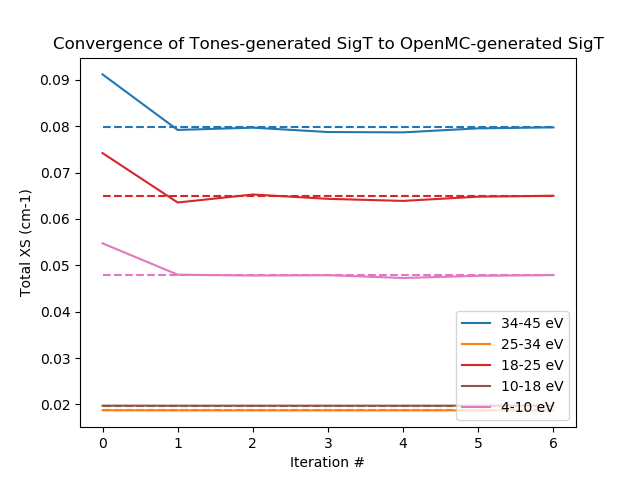
\includegraphics[width=0.6\textwidth]{convergence_of_tones_sigT}
    %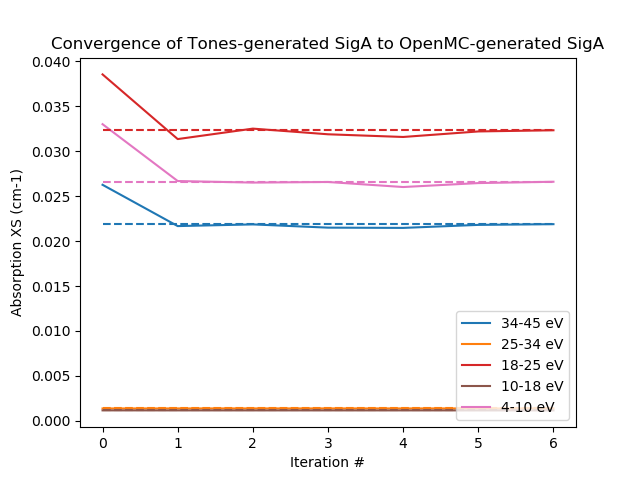
\includegraphics[width=0.6\textwidth]{convergence_of_tones_sigA}
    \includegraphics[width=0.6\textwidth]{tonesA_sigT}
    \includegraphics[width=0.6\textwidth]{tonesA_sigA}
      \caption{Shown above are the changes in $\Sigma_t,\Sigma_a$ over 9 iterations of Tone's method, plotted for 5 energy groups in the low resonance region. The solid lines represent values represented by Tone's method, while the dotted lines represent the values calculated by OpenMC. The values above were calculated using the problem specifications described in Sec.~\ref{enrichment}.}
      \label{fig:results1}
    \end{center}
  \end{figure}

  
%  \begin{figure}[H]
%    \begin{center}
%    \includegraphics[width=0.6\textwidth]{tonesA_sigT_ERROR}
%    \includegraphics[width=0.6\textwidth]{tonesA_sigA_ERROR}
%      \caption{Shown above are the percent errors for $\Sigma_t,\Sigma_a$ over 9 iteraiton of Tone's method, plotted for 5 energy groups in the low resonance region. The geometry is that described in Sec.~\ref{enrichment}.}
%      \label{fig:results2}
%    \end{center}
%  \end{figure}

 % Note that this comparison was also repeated, with the only difference in geometry being the creation of a hole in the center of the 3x3 grid. The geometry thus changed to what is shown in Fig.~\ref{fig:hole}

 %\begin{figure}
 %   \begin{center}
 %     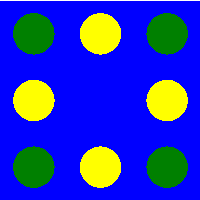
\includegraphics[width=0.3\textwidth]{hole_3x3}
 %     \caption{In addition to the system presented in Fig.~\ref{fig:geometry}, a 3x3 pin system with a hole in the center was considered. The enrichments and pin sizes all were held constant. This case is not presented further because its results are so close to those presented in Fig.~\ref{fig:results1} and Fig.~\ref{fig:results2} that any additional discussion would be repetitive.}
 %     \label{fig:hole}
 %   \end{center}
%\end{figure}




%%%%%%%%%%%%%%%%%%%%%%%%%%%%%%%%%%%%%%%%%%%%%%%%%%%%%%%%%%%%%%%%%%%%%%%%%%%%%%%
\section{Alternate Version of Tone's Method}
%%%%%%%%%%%%%%%%%%%%%%%%%%%%%%%%%%%%%%%%%%%%%%%%%%%%%%%%%%%%%%%%%%%%%%%%%%%%%%%
In Eq.~\ref{eq:tonesApprox}, we assumed that the fine energy term $\alpha$ was dependent on region $i$. Let's consider the case that, instead of $\alpha=\alpha_i(E)$, the assumptions is instead $\alpha=\alpha_j(E)$. In that case, Eq.~\ref{eq:tonesApprox} turns into
\begin{equation}\frac{P_{j\rightarrow i}(E)}{\Sigma_{t,i}(E)}=\alpha_{j}(E)\frac{P_{j\rightarrow i,g}}{\Sigma_{t,i,g}}\label{eq:tonesApprox2}.\end{equation}
Recall Eq.~\ref{eq:resultFromHetero},
\begin{equation*}\phi_{i}(E)=\frac{1}{E}\sum\limits_j\frac{P_{j\rightarrow i}(E)V_{j}\Sigma_{pot,j}}{\Sigma_{t,i}(E)V_{i}}\tag{\ref{eq:resultFromHetero}}.\end{equation*}
  Using Eq.~\ref{eq:tonesApprox2}, we can remove the energy dependence from $P_{j\rightarrow i}(E)$ and $\Sigma_{t,i}(E)$ in Eq.~\ref{eq:resultFromHetero},
\begin{equation}\phi_{i}(E)=\frac{1}{E}\sum\limits_j\frac{\alpha_j(E)P_{j\rightarrow i,g}V_{j}\Sigma_{pot,j}}{\Sigma_{t,i,g}V_{i}}.\label{eq:phiWithalphaj}\end{equation}
The problem here, however, is that since $\alpha_j(E)$ is dependent on $j$, we cannot remove it from the summation like we had done with the original Tone's derivation.So we must try to represent $\alpha_j(E)$ in terms of $\alpha_i(E)$.

Since we had assumed Eq.~\ref{eq:tonesApprox2} to be true, then we can reverse the indices to get
\begin{equation}\frac{P_{i\rightarrow j}(E)}{\Sigma_{t,j}(E)}=\alpha_{i}(E)\frac{P_{i\rightarrow j,g}}{\Sigma_{t,j,g}}\label{eq:something}.\end{equation}

Using the reciprocity relation from Eq.~\ref{eq:reciprocity}, we can rewrite the left side of Eq.~\ref{eq:something} to contain similar terms to those in Eq.~\ref{eq:tonesApprox2},
\begin{equation}P_{i\rightarrow j}(E)=\frac{P_{j\rightarrow i}(E)V_{j}\Sigma_{t,j}(E)}{V_{i}\Sigma_{t,i}(E)}\tag{\ref{eq:reciprocity}}\end{equation}


\begin{equation}\frac{P_{j\rightarrow i}(E)V_{j}\Sigma_{t,j}(E)}{V_{i}\Sigma_{t,i}(E)}\times\frac{1}{\Sigma_{t,j}(E)}=\alpha_{i}(E)\frac{P_{i\rightarrow j,g}}{\Sigma_{t,j,g}}\end{equation}

\begin{equation}\frac{P_{j\rightarrow i}(E)V_{j}}{V_{i}\Sigma_{t,i}(E)}=\alpha_{i}(E)\frac{P_{i\rightarrow j,g}}{\Sigma_{t,j,g}}\end{equation}
  Now we can plug $\alpha_j(E)$ into the above equation

\begin{equation}\frac{V_{j}}{V_{i}}\alpha_{j}(E)\frac{P_{j\rightarrow i,g}}{\Sigma_{t,i,g}}=\alpha_{i}(E)\frac{P_{i\rightarrow j,g}}{\Sigma_{t,j,g}}\end{equation}
  
\begin{equation}\alpha_{j}(E)=\alpha_{i}(E)\frac{P_{i\rightarrow j,g}}{\Sigma_{t,j,g}}\frac{\Sigma_{t,i,g}}{P_{j\rightarrow i,g}}\frac{V_{i}}{V_{j}}\end{equation}

  Now that we have $\alpha_j(E)$ in terms of $\alpha_i(E)$, we can plug this definition into Eq.~\ref{eq:phiWithalphaj} to get 

\begin{equation}\phi_{i}(E)=\frac{1}{E}\sum\limits_j\alpha_{i}(E)\frac{P_{i\rightarrow j,g}}{\Sigma_{t,j,g}}\frac{\Sigma_{t,i,g}}{P_{j\rightarrow i,g}}\frac{V_{i}}{V_{j}}\frac{P_{j\rightarrow i,g}V_{j}\Sigma_{pot,j}}{\Sigma_{t,i,g}V_{i}}\end{equation}
  \begin{equation}\phi_{i}(E)=\frac{1}{E}\sum\limits_j\alpha_{i}(E)\frac{P_{i\rightarrow j,g}\Sigma_{pot,j}}{\Sigma_{t,j,g}}\label{eq:again}\end{equation}


Now, just as in the original Tone's derivation, we need a better representation for $\alpha_i(E)$. We can attain this using the reciprocity relation and requirement for probabilities normalization, as had been done before.

  \begin{equation}\sum\limits_{j}\left(\frac{P_{j\rightarrow i}(E)V_{j}\Sigma_{t,j}(E)}{V_{i}\Sigma_{t,i}(E)}\right)=1\tag{\ref{eq:endOfReciprocity}}\end{equation}

    
    \begin{equation}\sum\limits_{j}\left(\alpha_j(E)\frac{P_{j\rightarrow i,g}V_{j}\Sigma_{t,j}(E)}{V_{i}\Sigma_{t,i,g}}\right)=1\end{equation}

      and we can use our definition of $\alpha_j(E)$ in terms of $\alpha_i(E)$ to get 
    \begin{equation}\sum\limits_{j}\left(\alpha_{i}(E)\frac{P_{i\rightarrow j,g}}{\Sigma_{t,j,g}}\frac{\Sigma_{t,i,g}}{P_{j\rightarrow i,g}}\frac{V_{i}}{V_{j}}\frac{P_{j\rightarrow i,g}V_{j}\Sigma_{t,j}(E)}{V_{i}\Sigma_{t,i,g}}\right)=1\end{equation}
    \begin{equation}\sum\limits_{j}\left(\alpha_{i}(E)\frac{P_{i\rightarrow j,g}\Sigma_{t,j}(E)}{\Sigma_{t,j,g}}\right)=1\end{equation}
      \begin{equation}\alpha_i(E)=\frac{1}{\sum\limits_{j}\frac{P_{i\rightarrow j,g}\Sigma_{t,j}(E)}{\Sigma_{t,j,g}}}\end{equation}
        Now we have an approxpriate definition of $\alpha_i(E)$ that we can use in Eq.~\ref{eq:again}
  \begin{equation}\phi_{i}(E)=\frac{1}{E}\frac{\sum\limits_j\left(P_{i\rightarrow j,g}\Sigma_{pot,j}\Big/\Sigma_{t,j,g}\right)}{\sum\limits_{j}\left(P_{i\rightarrow j,g}\Sigma_{t,j}(E)\Big/\Sigma_{t,j,g}\right)}\end{equation}
    \begin{equation}\phi_{i}(E)=\frac{1}{E}\frac{\sum\limits_j\left(P_{i\rightarrow j,g}N_{r,j}\sigma_{pot,r}\Big/\Sigma_{t,j,g}\right) +\sum\limits_j\left(P_{i\rightarrow j,g}\sum\limits_{k\neq r}N_{k,j}\sigma_{pot,k}\Big/\Sigma_{t,j,g}\right) }{
    \sum\limits_{j}\left(P_{i\rightarrow j,g}N_{r,j}\sigma_{t,r}(E)\Big/\Sigma_{t,j,g}\right) + \sum\limits_{j}\left(P_{i\rightarrow j,g}\sum\limits_{k\neq r}N_{k,j}\sigma_{t,k}(E)\Big/\Sigma_{t,j,g}\right)}\end{equation}
assuming that non-resonant nuclides only contribute potential scattering simlifies this to 
    \begin{equation}\phi_{i}(E)=\frac{1}{E}\frac{\sigma_{pot,r}\sum\limits_j\left(P_{i\rightarrow j,g}N_{r,j}\Big/\Sigma_{t,j,g}\right) +\sum\limits_j\left(P_{i\rightarrow j,g}\sum\limits_{k\neq r}N_{k,j}\sigma_{pot,k}\Big/\Sigma_{t,j,g}\right) }{
    \sigma_{t,r}(E)\sum\limits_{j}\left(P_{i\rightarrow j,g}N_{r,j}\Big/\Sigma_{t,j,g}\right) + \sum\limits_{j}\left(P_{i\rightarrow j,g}\sum\limits_{k\neq r}N_{k,j}\sigma_{pot,k}\Big/\Sigma_{t,j,g}\right)}\end{equation}




  \begin{equation}\phi_i(E)=\frac{1}{E}\frac{\sigma_{pot,r}+\sigma_{0}}{\sigma_{t,r}(E)+\sigma_{0}}~\mbox{where }\sigma_{0}=\frac{\sum\limits_j\sum\limits_{k\neq r}P_{i\rightarrow j,g}N_{k,j}\sigma_{pot,k}\Big/\Sigma_{t,j,g} }{\sum\limits_jP_{i\rightarrow j,g}N_{r,j}\Big/\Sigma_{t,j,g}}\label{eq:TonesB}\end{equation}
Note that Eq.~\ref{eq:TonesB} is very similar in form to Eq.~\ref{eq:Tones} (provided below). 
\begin{equation}\phi_i(E)=\frac{1}{E}\frac{\sigma_{pot,r}+\sigma_{0}}{\sigma_{t,r}(E)+\sigma_{0}}~\mbox{where }\sigma_{0}=\frac{\sum\limits_j\sum\limits_{k\neq r}P_{j\rightarrow i,g}V_{j}N_{k,j}\sigma_{pot,k}}{\sum\limits_jP_{j\rightarrow i,g}V_{j}N_{r,j}}\tag{\ref{eq:Tones}}\end{equation}
As mentioned in Sec.~\ref{sec:tone}, it is expected that the standard Tone's Method which uses the $\alpha_i(E)$ approximation is likely more accurate, since perserving information about the places of neutron absorption is so important for neutronics.


  \begin{figure}[H]
    \begin{center}
    %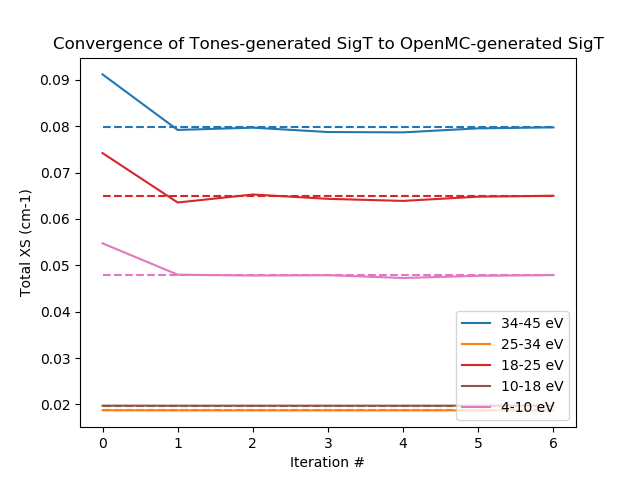
\includegraphics[width=0.6\textwidth]{convergence_of_tones_sigT}
    %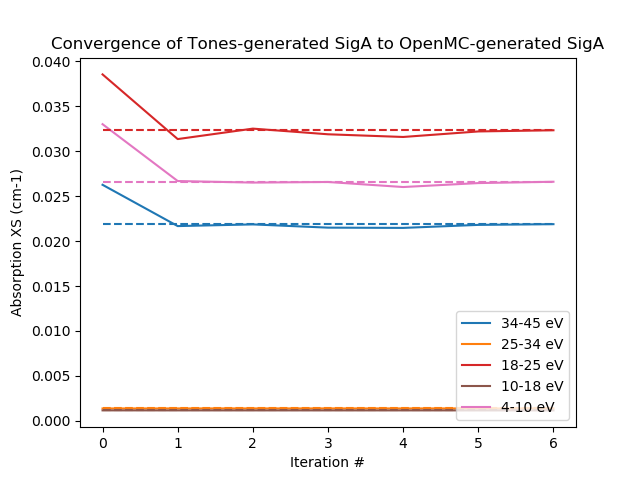
\includegraphics[width=0.6\textwidth]{convergence_of_tones_sigA}
    \includegraphics[width=0.49\textwidth]{tonesA_sigT}
    \includegraphics[width=0.49\textwidth]{tonesB_sigT}
    \includegraphics[width=0.49\textwidth]{tonesA_sigA}
    \includegraphics[width=0.49\textwidth]{tonesB_sigA}

    %\includegraphics[width=0.6\textwidth]{tonesA_sigA}
      \caption{Shown above are the changes in $\Sigma_t,\Sigma_a$ over 9 iterations of Tone's method, plotted for 5 energy groups in the low resonance region. The solid lines represent values represented by Tone's method, while the dotted lines represent the values calculated by OpenMC. The values above were calculated using the problem specifications described in Sec.~\ref{enrichment}.}
      \label{fig:results1}
    \end{center}
  \end{figure}

Surprisingly, both the standard and alternative form of the Tone's Method seem to perform very similarly for the test problem defined in Sec.~\ref{enrichment}. 

\begin{table}[H]
  \begin{center}
\begin{tabular}{|l|l|l|l|l|l|}\hline
  \multicolumn{6}{|c|}{$\Sigma_A [1/cm]$ values for various $E_g$, generated using standard and alternative Tone's Method} \\\hline
           &34-45 eV& 25-34 eV   & 18-25 eV   & 10-18 eV & 4-10 eV \\\hline
  Standard   & 0.0222826 & 0.00138918 & 0.0325555 & 0.00117075 & 0.02633830 \\\hline
  Alternative& 0.0232309 & 0.00138892 & 0.0337358 & 0.00117093 & 0.02757813\\\hline&&&&&\\[1pt]\hline
  \multicolumn{6}{|c|}{$\Sigma_T [1/cm]$ values for various $E_g$, generated using standard and alternative Tone's Method} \\\hline
           &34-45 eV& 25-34 eV   & 18-25 eV   & 10-18 eV & 4-10 eV \\\hline
  Standard $\alpha_i(E)$ approx.  & 0.0808003 & 0.01870110& 0.0653392& 0.01971423 &  0.04761292\\\hline
  Alternative $\alpha_j(E)$ approx.& 0.0832751& 0.01870265& 0.0670886& 0.01971482&0.04893870\\\hline


\end{tabular}
    \caption{$\sigma_0$ values (in barns)  uesd for generating dilution table. Note that increased fineness in grid for values in the 10's to 1000's region. The choice to do so was due to the behavior observed in Fig.~\ref{fig:dependencyOnBackground}.}
  \end{center}
\end{table}


  \newpage




  \bibliographystyle{unsrt}
\bibliography{notes}
\end{document}
















